\documentclass{beamer}
\usepackage{graphicx}
\usepackage{booktabs}
\usepackage{tcolorbox}
\usepackage{amsmath, esint}
\usepackage{tikz}
\usetikzlibrary{backgrounds, positioning, arrows, scopes, shapes, shapes.misc, shapes.multipart}
\tikzset{
    cross/.style={cross out, draw=black, minimum size=2*(#1-\pgflinewidth), inner sep=0pt, outer sep=0pt},
    cross/.default={10pt},
    split/.style={rectangle split, rectangle split parts=7, draw, inner sep=0ex, rectangle split horizontal, minimum size=4ex},
    textstyle/.style={text height=1.5ex, text depth=.25ex}
}

\usepackage{amsthm}
\usepackage{amstext}
\usepackage{amssymb}
%%\usepackage[plain]{algorithm}
%%\usepackage{algpseudocode}

\usepackage{minted}
\usepackage{xcolor} 
\definecolor{LightGray}{gray}{0.975}

%\usetheme{Warsaw}
\usefonttheme{serif} 

\title[L5 DP]{Introduction to Algorithms \\ Lecture 5: Dynamic Programming (DP)}
\author{Prof. Charles E. Leiserson and Prof. Erik Demaine \\ Massachusetts Institute of Technology}
\date{\today}

\setbeamertemplate{navigation symbols}{}%remove navigation symbols

\defbeamertemplate*{footline}{shadow theme}{%
    \leavevmode%
    \hbox{
        \begin{beamercolorbox}[wd=.5\paperwidth,ht=2.5ex,dp=1.125ex,leftskip=.3cm plus1fil,rightskip=.3cm]{author in head/foot}%
            \usebeamerfont{author in head/foot} Introduction to Algorithms: \hfill \insertshorttitle
        \end{beamercolorbox}%
        \begin{beamercolorbox}[wd=.5\paperwidth,ht=2.5ex,dp=1.125ex,leftskip=.3cm,rightskip=.3cm plus1fil]{title in head/foot}%
            \usebeamerfont{title in head/foot} \hfill \insertframenumber\,/\,\inserttotalframenumber%
        \end{beamercolorbox}
    }%
    \vskip0pt%
}

\AtBeginSection[]{
    \begin{frame}<beamer>
    \frametitle{Plan}
    \tableofcontents[currentsection]
    \end{frame}
}

\begin{document}

\frame{\titlepage}

\begin{frame}{Introduction to Algorithms}
    \centering
    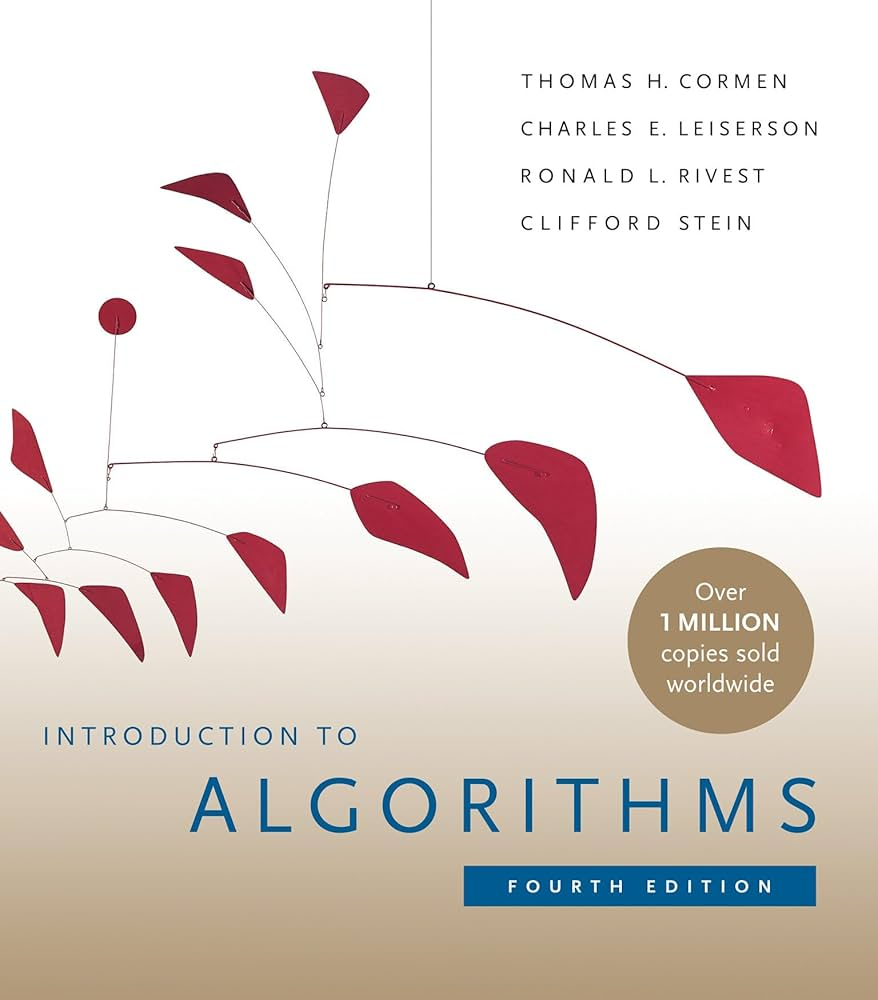
\includegraphics[width=0.45\textwidth]{figures/book_cover.jpg} \\
    \vspace{5mm}{
        \tiny
        Content has been extracted from \textit{Introduction to Algorithms}, Fourth Edition, by Cormen, Leiserson, Rivest, and Stein. MIT Press. 2022.\\
        Visit \url{https://mitpress.mit.edu/9780262046305/introduction-to-algorithms/}.\\
        Original slides from \textit{Introduction to Algorithms 6.046J/18.401J}, Fall 2005 Class by Prof. Charles Leiserson and Prof. Erik Demaine. MIT OpenCourseWare Initiative available at \url{https://ocw.mit.edu/courses/6-046j-introduction-to-algorithms-sma-5503-fall-2005/}.\\
    }
\end{frame}

\section{Dynamic Programming}

\begin{frame}{Dynamic Programming\footnote{\textit{Programming} in this context refers to a tabular method, not to writing computer code.} (DP)}
    \begin{itemize}
        \item Invented by Richard Bellman in 1950s.
        \item Desing technique, like Divide \& Conquer.
        \item Applies when the subproblems overlap --that is, when subproblems share subsubproblems.
        \item It solves each subsubproblem just once and then saves its answer in a table.
        \item DP typically applies to optimization problems:
        \begin{itemize}
            \item have many possible solutions.
            \item find a solution with the optimal (min or max) value.
            \item \textit{an} optimal solution, not \textit{the} optimal solution.
        \end{itemize}
    \end{itemize}
\end{frame}

\begin{frame}{DP notions}
    \begin{enumerate}
        \item Characterize the structure of an optimal solution.
        \item Recursively define the value of an optimal solution based on optimal solutions of subproblems.
        \item Compute the value of an optimal solution in bottom-up fashion (recursion \& memoization).
        \item Construct an optimal solution from the computed information.
    \end{enumerate}
    \vspace{10mm}
    \centering
    \Large
    \textcolor{blue}{\textbf{DP}} = \textcolor{orange}{\textbf{Recursion}} + \textcolor{olive}{\textbf{Memoization}}
\end{frame}

\begin{frame}{DP notions}
    \centering
    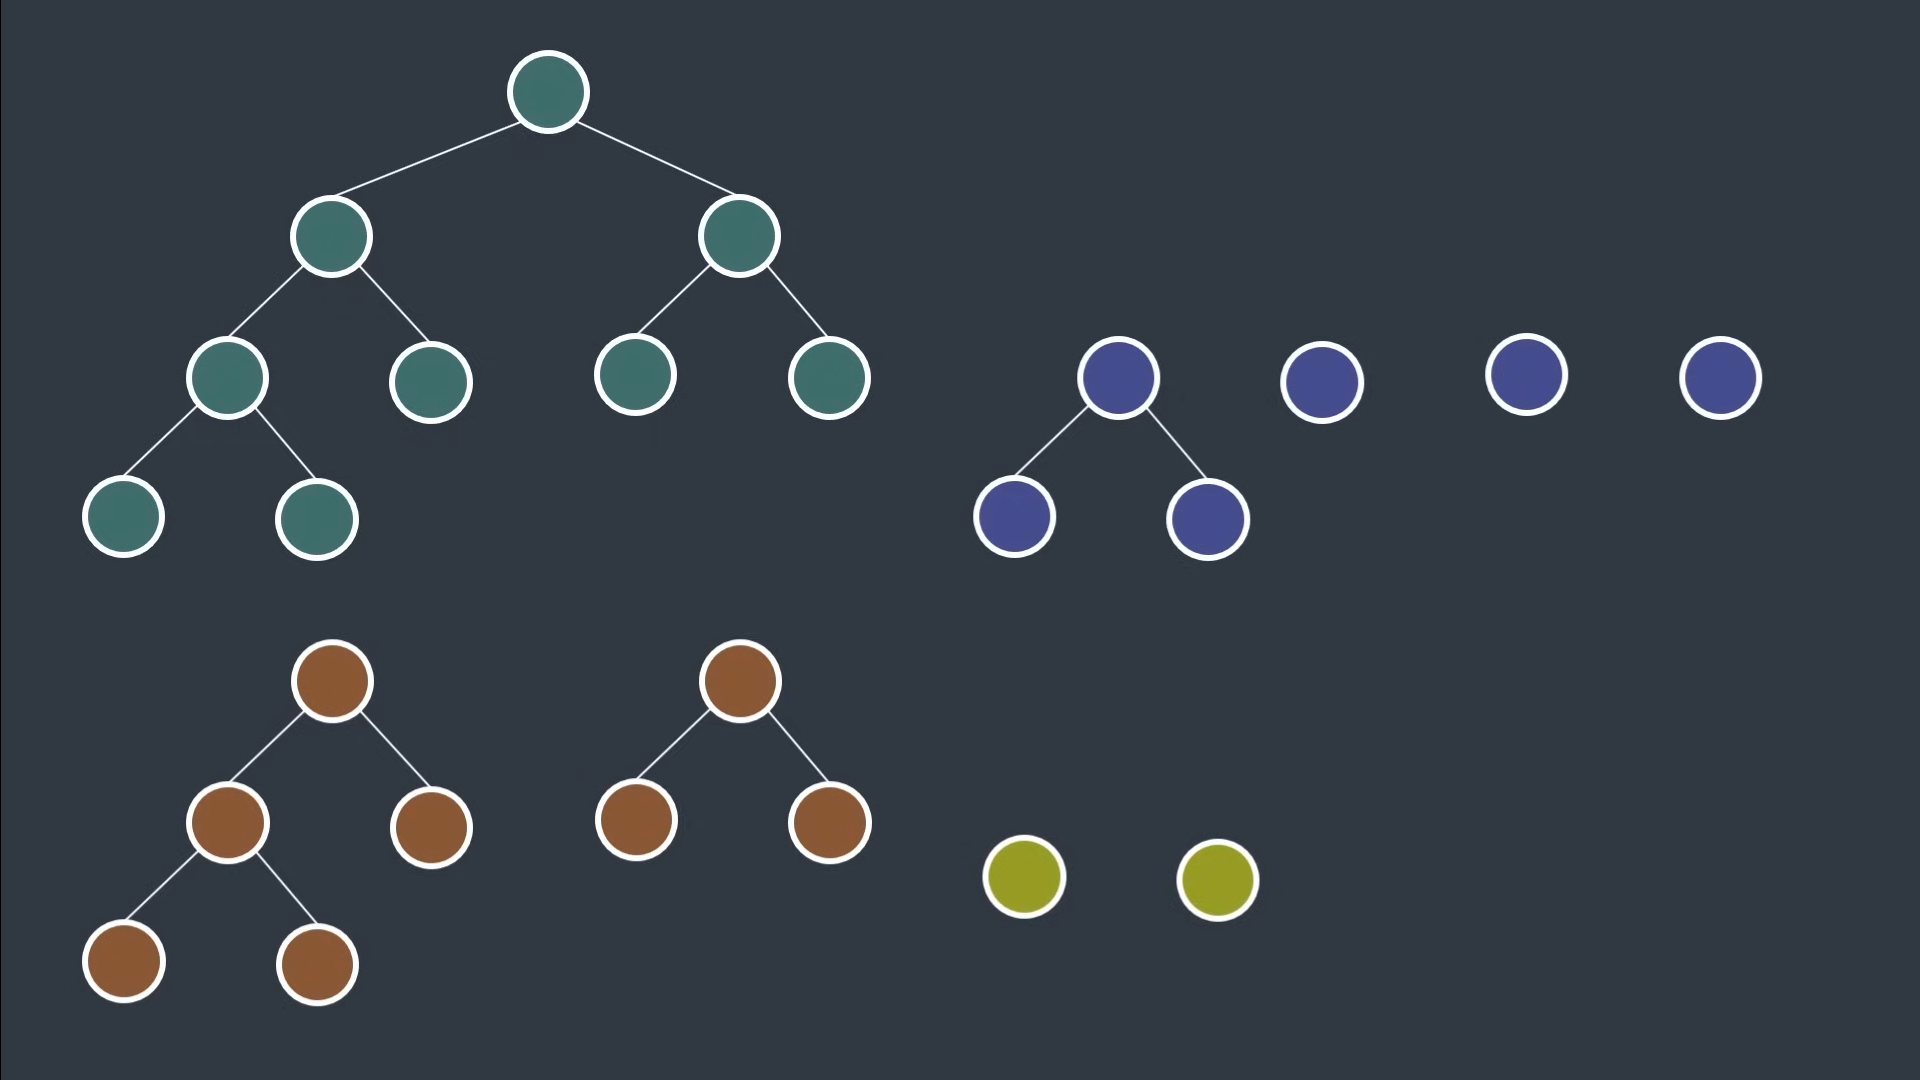
\includegraphics[width=\textwidth]{figures/dp01.png}
\end{frame}

\begin{frame}{N-th Fibonacci Number\footnote{\scriptsize \textit{Mastering Dynamic Programming - How to solve any interview problem (Part 1)}. Tech With Nikola Channel, 2024. YouTube, available at \url{https://youtu.be/Hdr64lKQ3e4?si=ycTe-hoyfaICRWXt}}}
    Write a function that returns the n-th Fibonacci number.
    \begin{equation*}
        \begin{align*}
            F_1 &= F_2 = 1 \\
            F_n &= F_{n - 1} + F_{n - 2} \\
        \end{align*}
    \end{equation*}
    \centering
    \LARGE
    \begin{tabular}{| c | c | c | c | c | c | c | c |} \hline
        n & 1 & 2 & 3 & 4 & 5 & 6 & 7  \\ \hline
    $F_n$ & 1 & 1 & 2 & 3 & 5 & 8 & 13 \\ \hline
    \end{tabular}
\end{frame}

\begin{frame}[fragile]{Naive Approach}
    \begin{minted}
    [tabsize=4, obeytabs, frame=lines, framesep=2mm, baselinestretch=1.2, bgcolor=LightGray, fontsize=\scriptsize, linenos]{python}
    def fib(n):
        if n <= 2:
            result = 1
        else:
            result = fib(n - 1) + fib(n - 2)
        return result
    \end{minted}
    \pause
    \begin{minted}
    [tabsize=4, obeytabs, framesep=2mm, baselinestretch=1.2, bgcolor=LightGray, fontsize=\scriptsize]{text}
    print(fib(7))
    Output: 13
    print(fib(50))
    Output: ???
    \end{minted}
\end{frame}

\begin{frame}{Naive Approach}
    \centering
    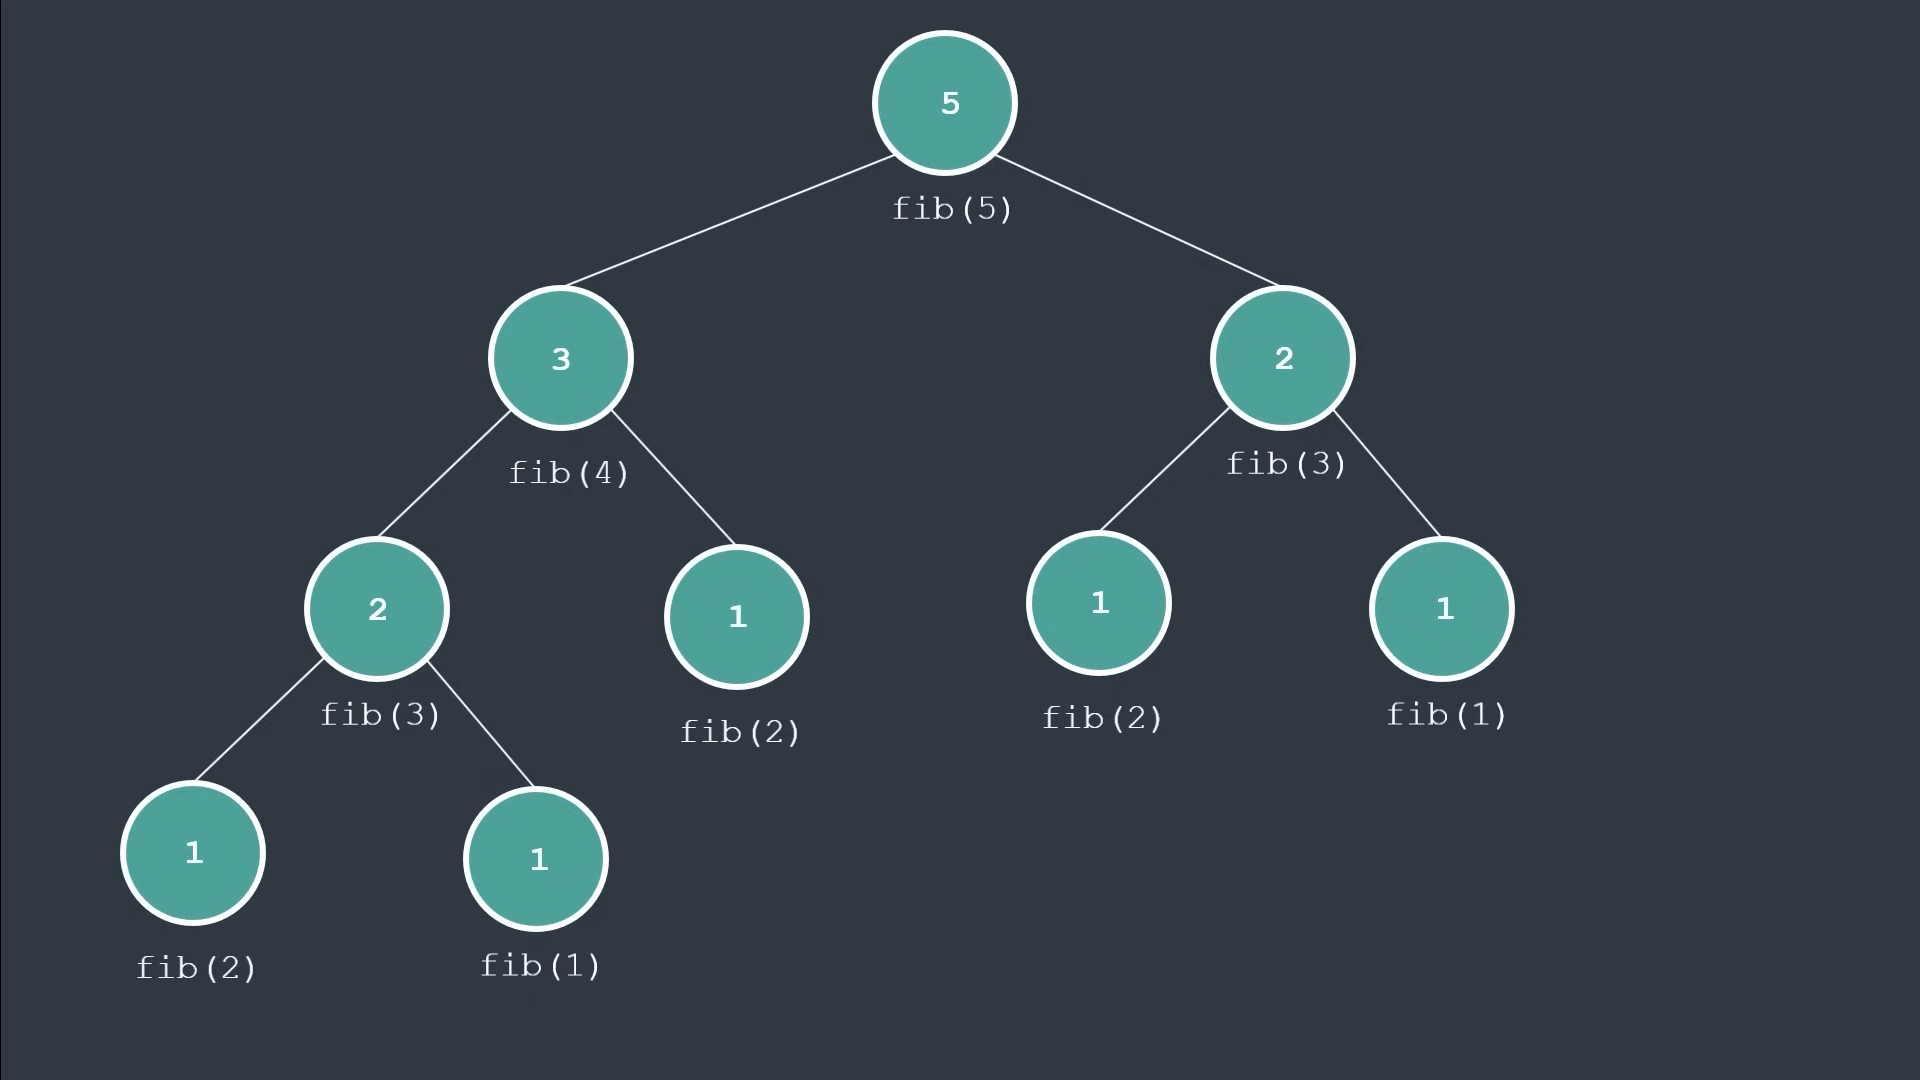
\includegraphics[width=\textwidth]{figures/fb01.png}
\end{frame}
\begin{frame}{Naive Approach}
    \centering
    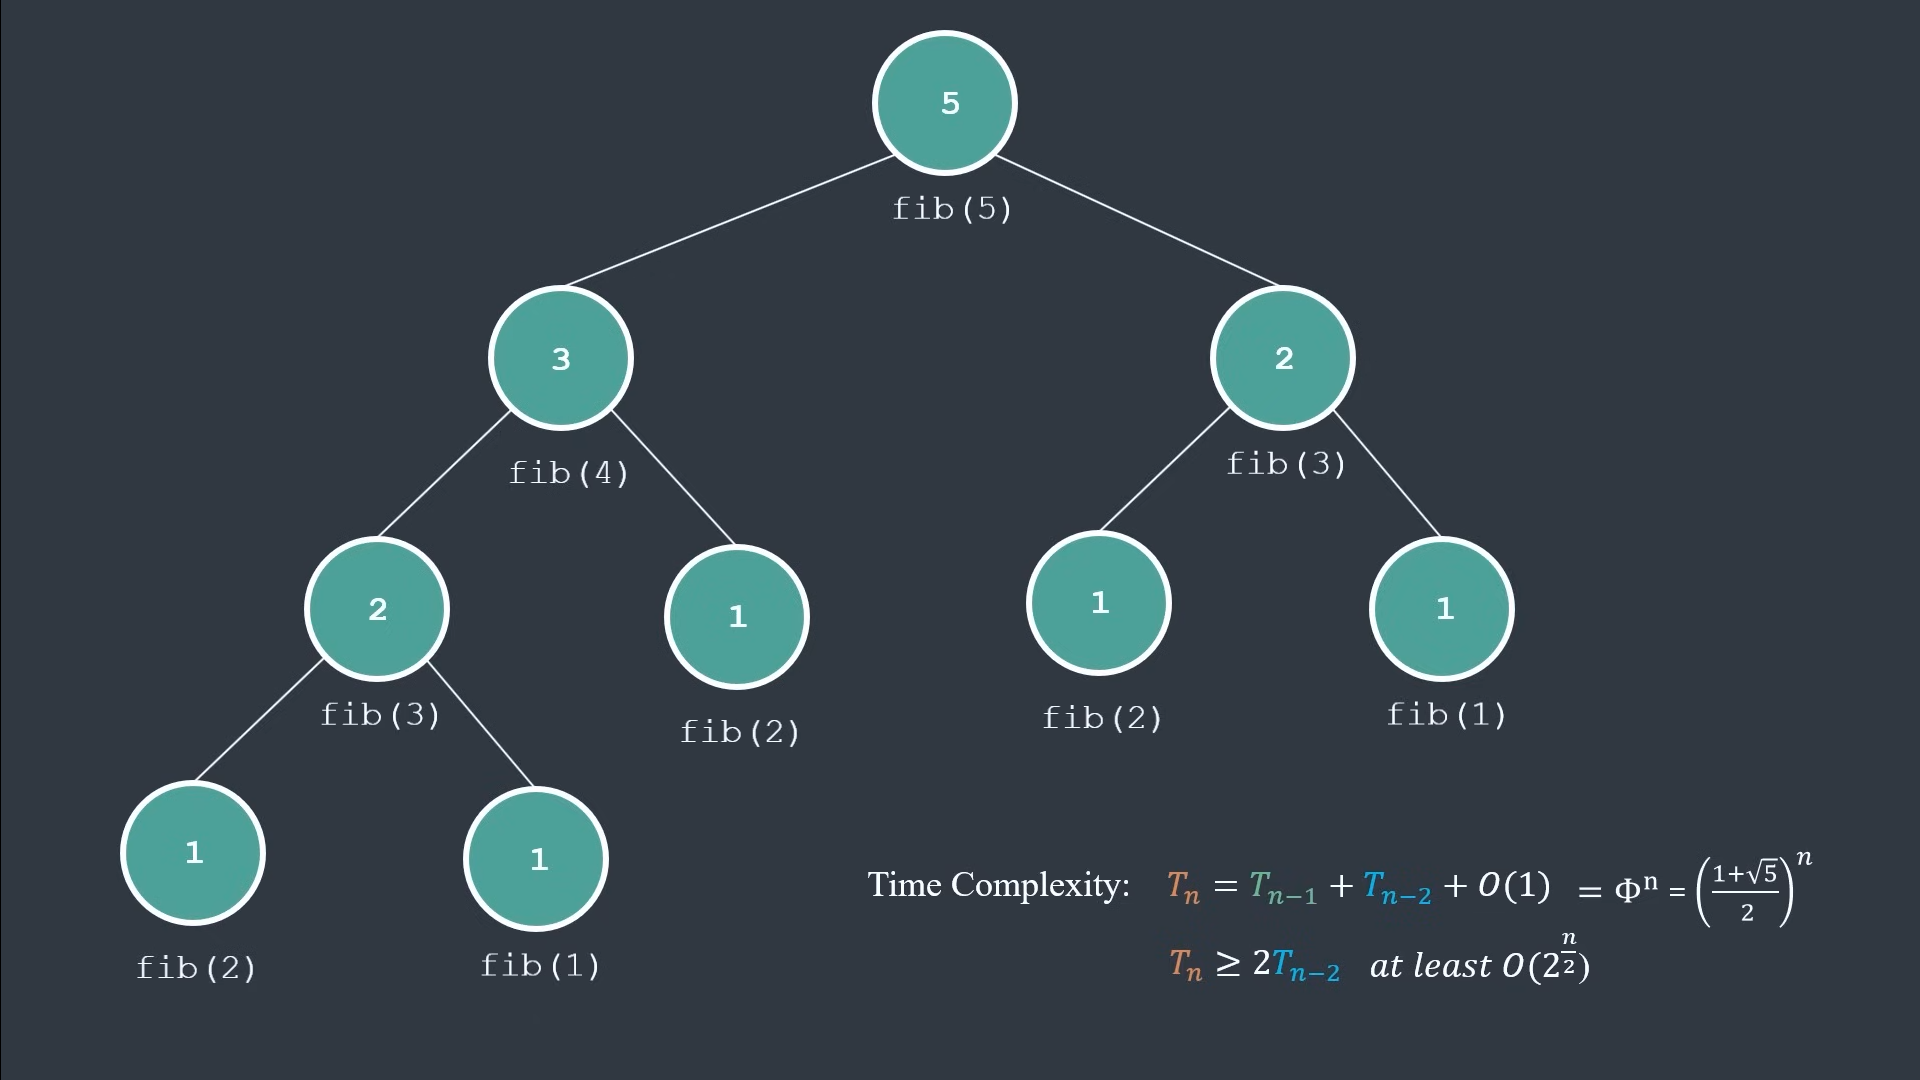
\includegraphics[width=\textwidth]{figures/fb02.png}
\end{frame}
\begin{frame}{Naive Approach}
    \centering
    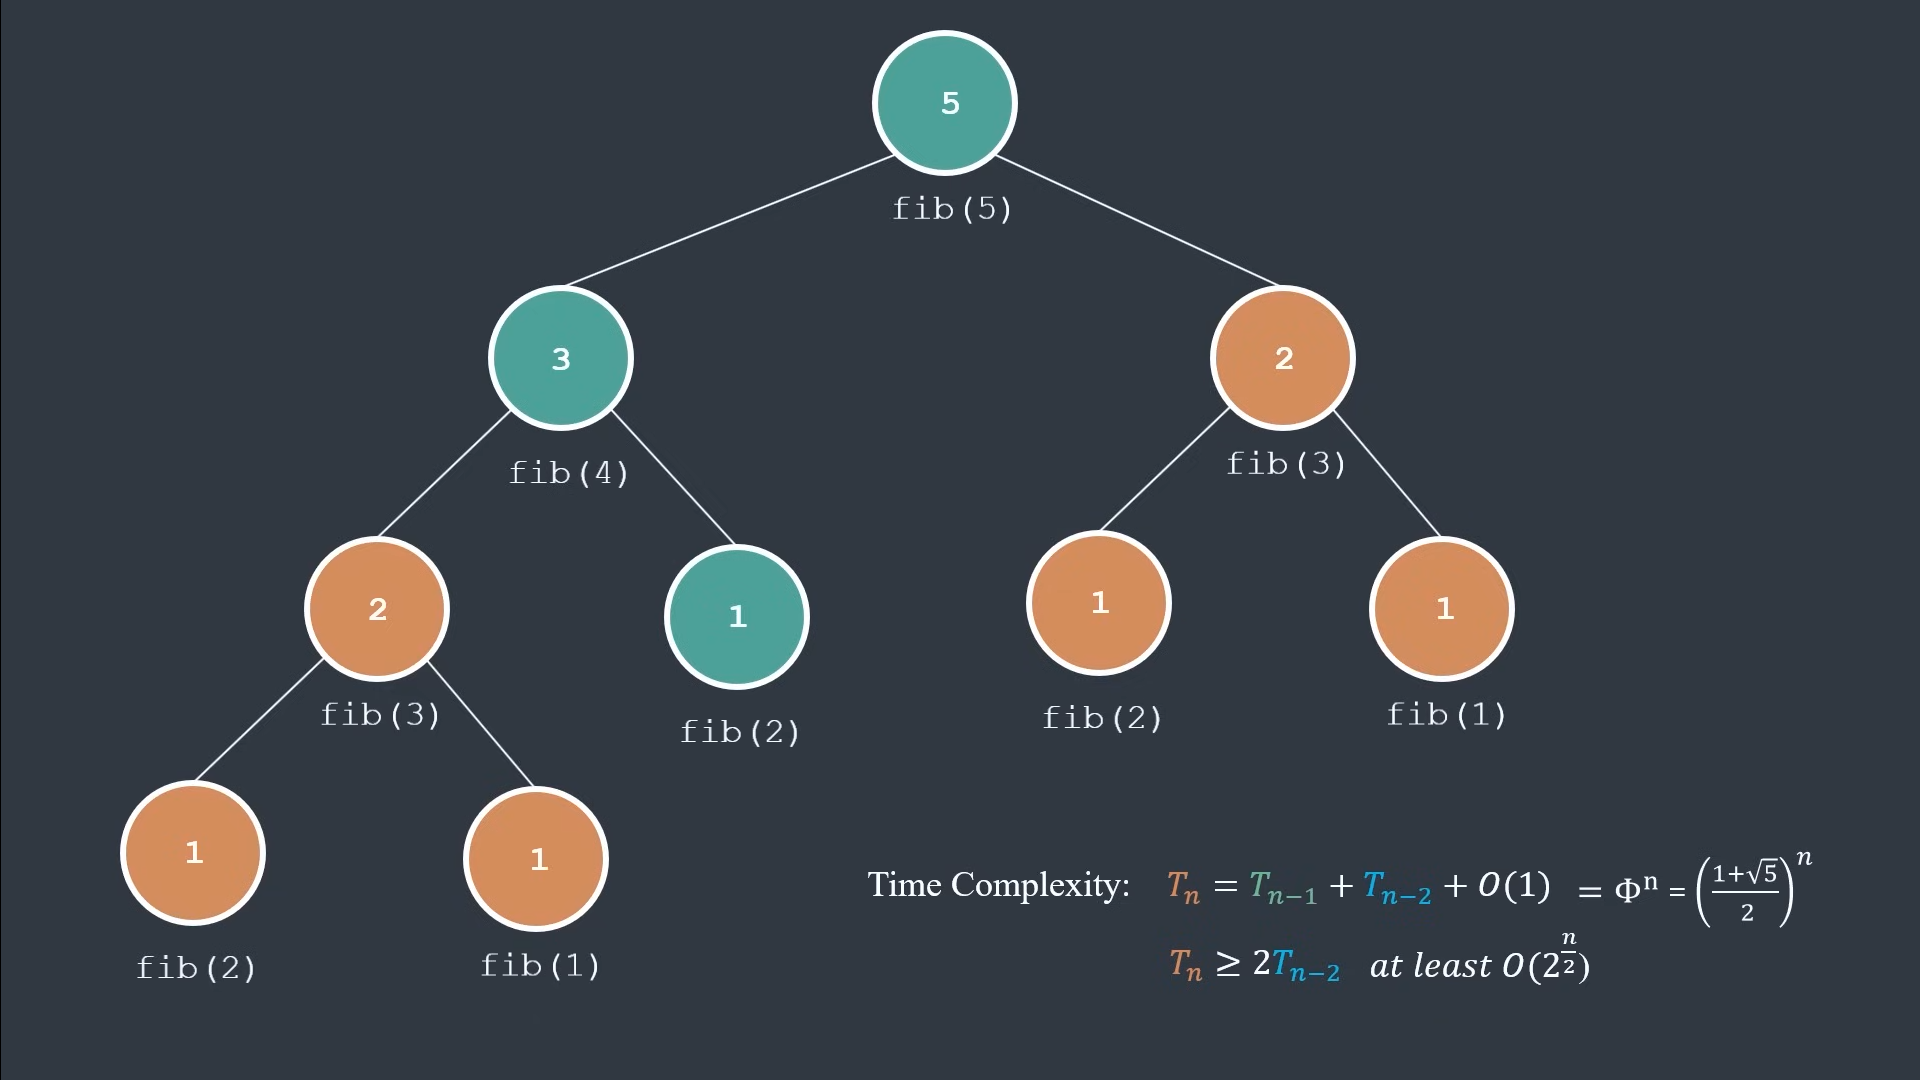
\includegraphics[width=\textwidth]{figures/fb03.png}
\end{frame}
\begin{frame}{Naive Approach}
    \centering
    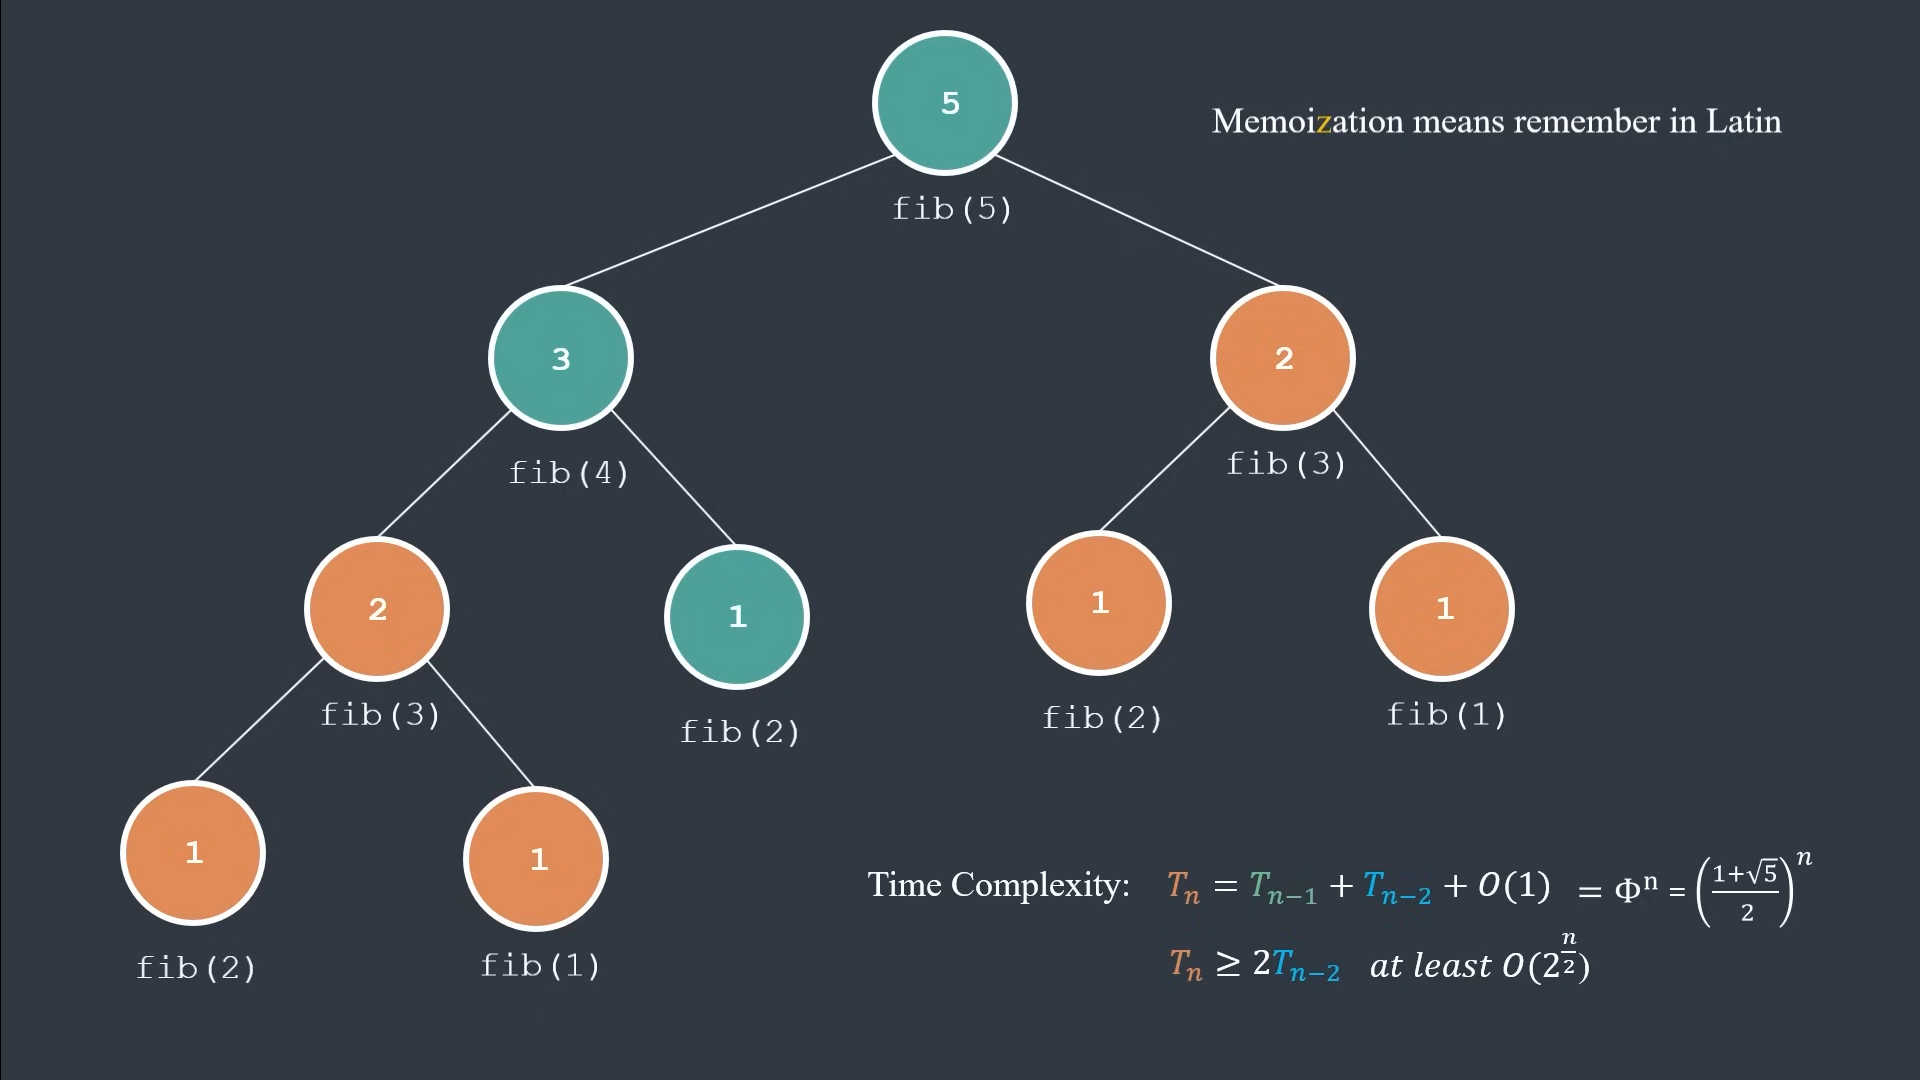
\includegraphics[width=\textwidth]{figures/fb04.png}
\end{frame}

\begin{frame}[fragile]{Memoization Approach}
    \begin{minted}
    [tabsize=4, obeytabs, frame=lines, framesep=2mm, baselinestretch=1.2, bgcolor=LightGray, fontsize=\scriptsize, linenos]{python}
    memo = {} # adding a dictionary...
    def fib(n):
        if n in memo: # asking if n is in dict...
            return memo[n] # if so, we are done!
        if n <= 2:
            result = 1
        else:
            result = fib(n - 1) + fib(n - 2)
        return result
    \end{minted}
    \pause
    \begin{minted}
    [tabsize=4, obeytabs, framesep=2mm, baselinestretch=1.2, bgcolor=LightGray, fontsize=\scriptsize]{text}
    print(fib(7))
    Output: 13
    print(fib(50))
    Output: 12586269025
    \end{minted}
    \pause
    \Large
    Time Complexity: $O(n)$.
\end{frame}

\begin{frame}{ }
    \centering
    \LARGE
    \textcolor{blue}{\textbf{DP}} = \textcolor{orange}{\textbf{Recursion}} + \textcolor{olive}{\textbf{Memoization}}
\end{frame}

\begin{frame}[fragile]{Bottom-up Approach}
    \begin{minted}
    [tabsize=4, obeytabs, frame=lines, framesep=2mm, baselinestretch=1.2, bgcolor=LightGray, fontsize=\scriptsize, linenos]{python}
    def fib(n):
        memo = {}
        for i in range(1, n + 1):
            if i <= 2:
                result = 1
            else:
                result = memo[n - 1] + memo[n - 2]
            memo[i] = result
        return memo[n]
    \end{minted}
\end{frame}

\begin{frame}{ }
    \centering
    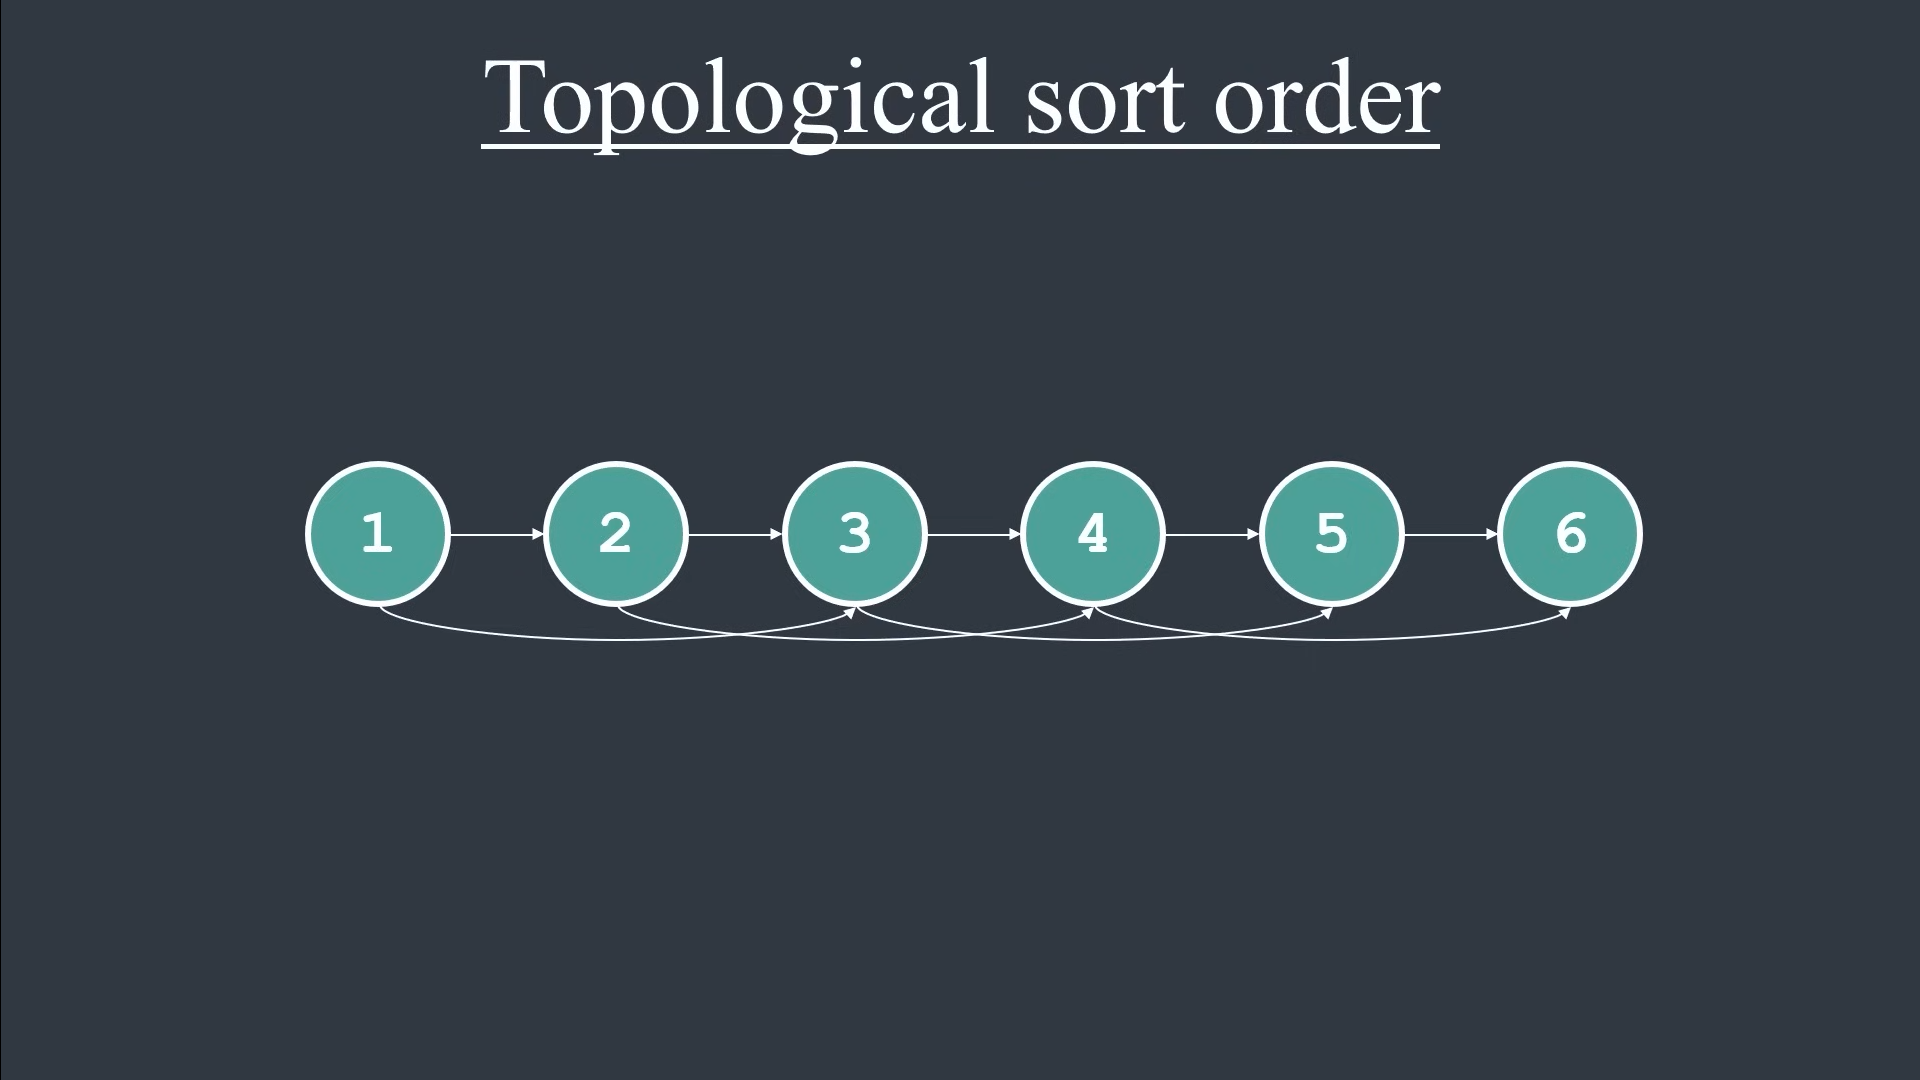
\includegraphics[width=\textwidth]{figures/topo.png}
\end{frame}

\begin{frame}{Longest Palindromic Sequence}
    \begin{exampleblock}{Definition:}
        A palindrome is a string that is unchanged when reversed.
    \end{exampleblock}
    \begin{itemize}
     \item Examples: \texttt{radar}, \texttt{civic}, \texttt{t}, \texttt{bb}, \texttt{redder}.
     \item Given: A string $X[1 \ldots n]$, $n \geq 1$.
     \item To find: Longest palindrome that is a subsequence.
     \item Example: Given ``c h a r a c t e r''.
     \item Output: ``c a r a c''.
     \item Answer will be $\geq 1$ in length.
    \end{itemize}
\end{frame}

\begin{frame}[fragile]{Strategy}
    $L(i, j)$: length of longest palindromic subsequence of $X[i \ldots j]$ for $i \leq j$.
    \begin{minted}
    [tabsize=4, obeytabs, frame=lines, framesep=2mm, baselinestretch=1.2, bgcolor=LightGray, fontsize=\scriptsize, linenos]{python}
    def L(i, j):
        if i == j:
            return 1
        if X[i] == X[j]:
            if i + 1 == j:
                return 2
            else:
                return 2 + L(i + i, j - 1)
        else:
            return max( L(i + 1, j), L(i, j - 1) )
    \end{minted}
\end{frame}

\begin{frame}{Analysis}
    As written, program can run in exponential time: suppose all symbols $X[i]$ are distinct.
    \begin{equation*}
        \begin{align*}
            T(n) &= \text{running time on input of length } n \\
            T(n) &=
                    \begin{cases}
                        1         & n = 1 \\
                        2T(n - 1) & n > 1 \\
                    \end{cases} \\
                 &= 2^{n - 1}
        \end{align*}
    \end{equation*}
\end{frame}










\begin{frame}{}
\end{frame}

\begin{frame}{}
%    \begin{minted}
%    [tabsize=4, obeytabs, frame=lines, framesep=2mm, baselinestretch=1.2, bgcolor=LightGray, fontsize=\scriptsize]{sql}
%    \end{minted}
\end{frame}

\begin{frame}{}
    \centering
    \Huge End of Lecture 5.
\end{frame}

\section*{Takeaways}

% Tim Duncan's Top 5 Fundamental Takeaways of the Today's Class
% \begin{frame}{TDT5FTOTTC}
%     \centering
%     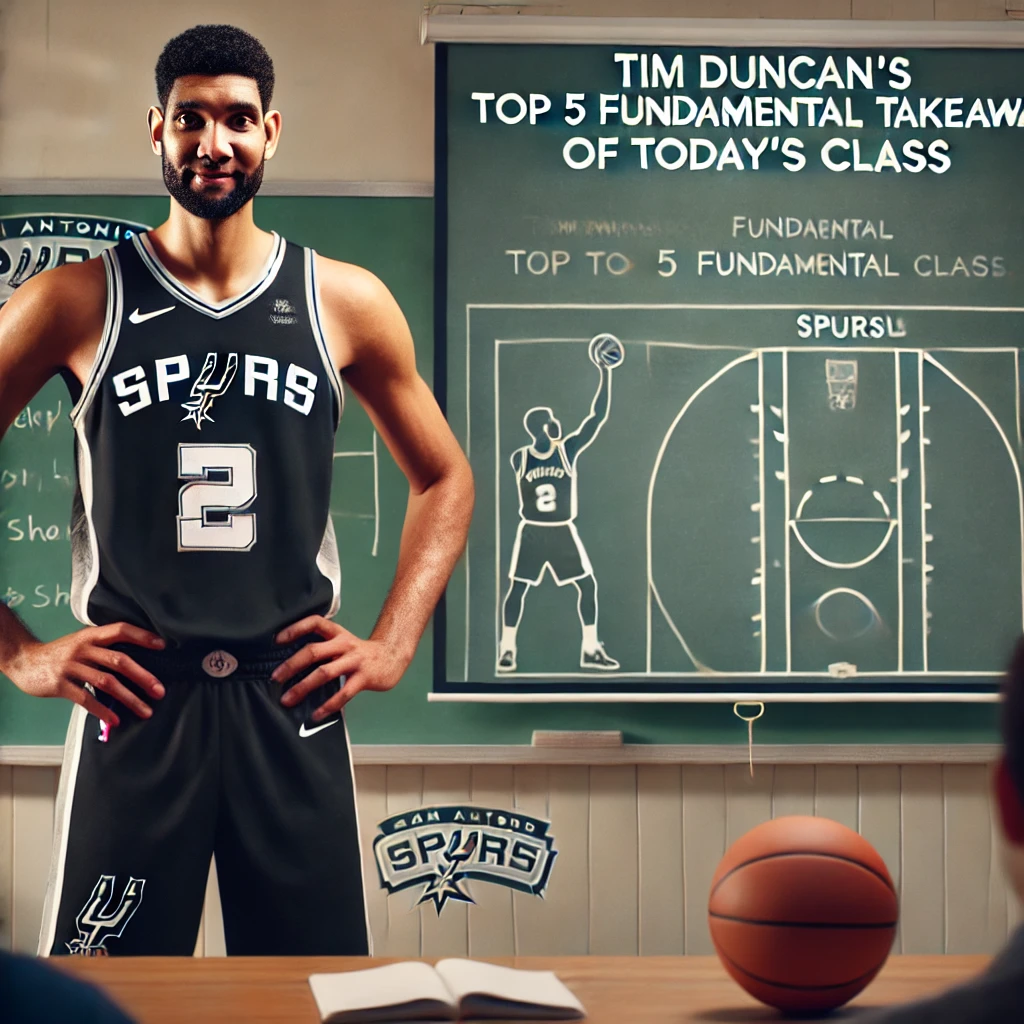
\includegraphics[width=0.75\textwidth]{figures/tim.png}
% \end{frame}
%
% \begin{frame}{Top 5 Fundamental Takeaways}
%     \small
%     \begin{enumerate} \pause
%         \item[5] \textbf{Quicksort is a Divide-and-Conquer Algorithm} – It recursively partitions an array around a pivot and sorts the subarrays efficiently.\pause
%
%         \item[4] \textbf{Partitioning is the Core of Quicksort} – The partitioning step ensures elements are correctly placed around the pivot in $O(n)$ time.\pause
%
%         \item[3] \textbf{Best-case and Worst-case Analysis} – Quicksort runs in $O(n \log n)$ in the best case but can degrade to $O(n^2)$ if poorly partitioned.\pause
%
%         \item[2] \textbf{Randomized Quicksort Helps Avoid Worst-case Behavior} – Choosing a random pivot prevents consistently bad splits and ensures an expected $O(n \log n)$ runtime.\pause
%
%         \item[1] \textbf{Quicksort is Highly Efficient in Practice} – It outperforms merge sort in most cases and benefits from hardware optimizations.
%
%     \end{enumerate}
% \end{frame}

\begin{frame}{Introduction to Algorithms}
    \centering
    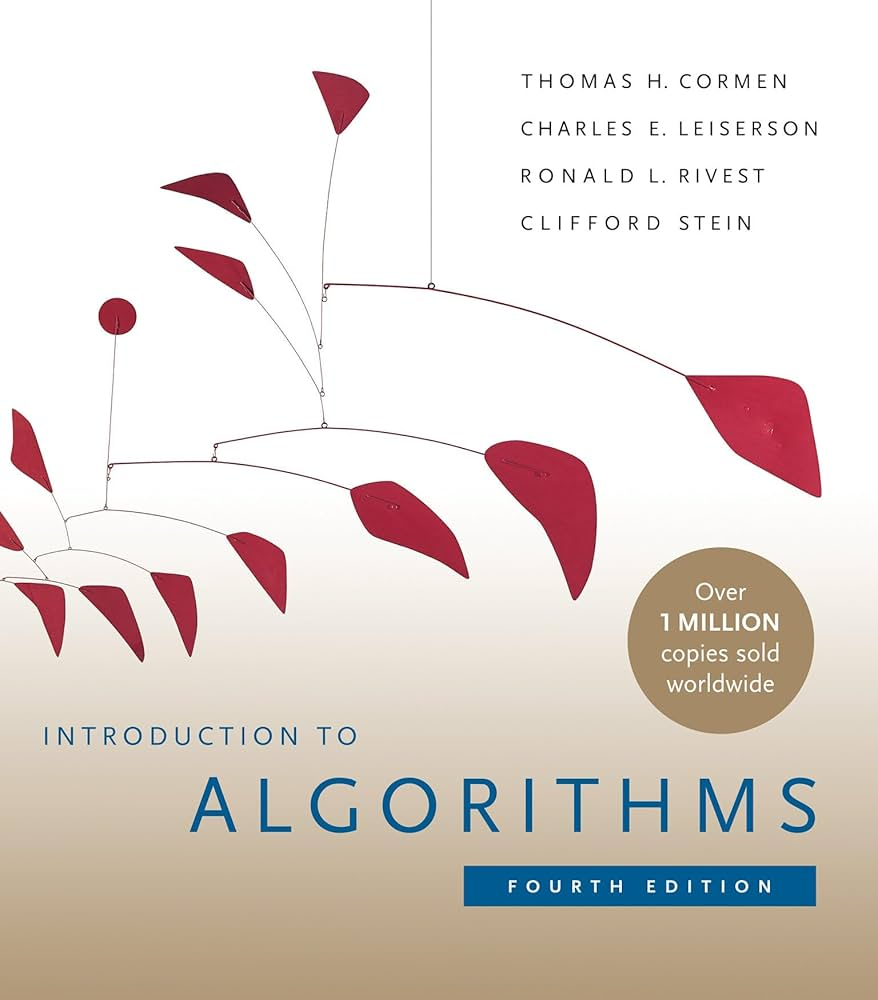
\includegraphics[width=0.45\textwidth]{figures/book_cover.jpg} \\
    \vspace{5mm}{
        \tiny
        Content has been extracted from \textit{Introduction to Algorithms}, Fourth Edition, by Cormen, Leiserson, Rivest, and Stein. MIT Press. 2022.\\
        Visit \url{https://mitpress.mit.edu/9780262046305/introduction-to-algorithms/}.\\
        Original slides from \textit{Introduction to Algorithms 6.046J/18.401J}, Fall 2005 Class by Prof. Charles Leiserson and Prof. Erik Demaine. MIT OpenCourseWare Initiative available at \url{https://ocw.mit.edu/courses/6-046j-introduction-to-algorithms-sma-5503-fall-2005/}.\\
    }
\end{frame}

\end{document}
